\section{Pruning}
Pruning is a model compression technique that removes weights while minimally affecting the model's accuracy.
Depending on the specific model, more or less pruning can be performed without significant loss in accuracy.
Pruning can significantly reduce the number of (unique) weights to be configured.
A prune percentage of 80\% is not uncommon and this directly translates to 80\% less (unique) weights to be configured.

Since pruning only affects the \textit{weights} data section of the compiled model, which is in a lot of cases the largest data section, it significantly affects the total data size of the compiled model.
Not only is this advantageous for less data transfer during a configuration, a smaller model size also allows for a greater freedom for the compiler to search for a more performant mapping.

If we have a model with different prune levels and a similar mapping, we can simply compute the amount of data to write with:
\begin{equation}
    d_\textrm{total} = (1-p) \times d_\textrm{weights} + d_\textrm{masks} + d_\textrm{states} + d_\textrm{axons} + d_\textrm{headers}
\end{equation}

Let's take the \textit{mobnetv2} model as an example.
Without any pruning applied, a mapping requires a total of \num{4166408} bytes for the weights.
A pruning of 80\% applied to the weights gives us a total configuration data reduction of 12\% (see \cref{fig:mobnetv2_prune_vs_data}).
If the states are excluded, the reduction in the amount of configuration data read is almost doubled.
In terms of energy, the configuration energy, with 80\% pruning and no transferring of states, is reduced with 43\%.  

\begin{figure}[hbtp]
\centering
    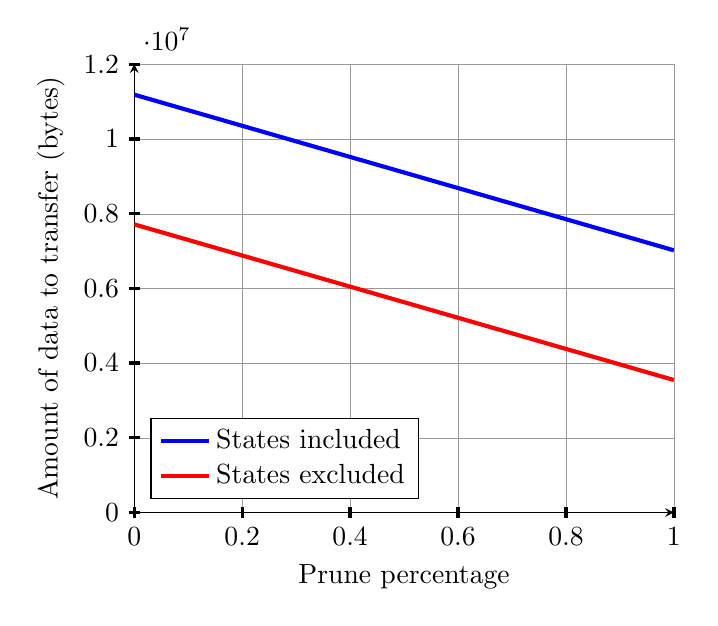
\begin{tikzpicture}
        \begin{axis}[
            axis lines = left,
            xlabel = {Prune percentage},
            ylabel = {Amount of data to transfer (bytes)},
            ymin = 0, ymax = 12e6,
            xmin = 0, xmax = 1,
            grid=both,
            grid style={line width=.1pt, draw=gray!80},
            every major tick/.append style={very thick, major tick length=4pt, black},
            legend cell align=left,
                legend pos=south west,
        ]
        \addplot [
            domain=0:1, 
            samples=2, 
            color=blue,
            line width=1.5pt,
        ]
        {(1-x)*4166408 + 1008312 + 1009248 + 1528928 + 3471616};
        
        \addplot [
            domain=0:1, 
            samples=2, 
            color=red,
            line width=1.5pt
        ]
        {(1-x)*4166408 + 1008312 + 1009248 + 1528928};
        
        
        \legend{States included,States excluded}
        
        
        \end{axis}
    \end{tikzpicture}
\caption{The configuration data read from external memory of the \textit{mobnetv2} model with different prune levels}
\label{fig:mobnetv2_prune_vs_data}
\end{figure}

Pruning can significantly reduce the energy consumption for configuration. 
However, the amount of pruning that can be applied is dependent on the specific model in question and the accuracy required.
